% Options for packages loaded elsewhere
\PassOptionsToPackage{unicode}{hyperref}
\PassOptionsToPackage{hyphens}{url}
\PassOptionsToPackage{dvipsnames,svgnames,x11names}{xcolor}
%
\documentclass[
  letterpaper,
  DIV=11,
  numbers=noendperiod]{scrartcl}

\usepackage{amsmath,amssymb}
\usepackage{iftex}
\ifPDFTeX
  \usepackage[T1]{fontenc}
  \usepackage[utf8]{inputenc}
  \usepackage{textcomp} % provide euro and other symbols
\else % if luatex or xetex
  \usepackage{unicode-math}
  \defaultfontfeatures{Scale=MatchLowercase}
  \defaultfontfeatures[\rmfamily]{Ligatures=TeX,Scale=1}
\fi
\usepackage{lmodern}
\ifPDFTeX\else  
    % xetex/luatex font selection
\fi
% Use upquote if available, for straight quotes in verbatim environments
\IfFileExists{upquote.sty}{\usepackage{upquote}}{}
\IfFileExists{microtype.sty}{% use microtype if available
  \usepackage[]{microtype}
  \UseMicrotypeSet[protrusion]{basicmath} % disable protrusion for tt fonts
}{}
\makeatletter
\@ifundefined{KOMAClassName}{% if non-KOMA class
  \IfFileExists{parskip.sty}{%
    \usepackage{parskip}
  }{% else
    \setlength{\parindent}{0pt}
    \setlength{\parskip}{6pt plus 2pt minus 1pt}}
}{% if KOMA class
  \KOMAoptions{parskip=half}}
\makeatother
\usepackage{xcolor}
\setlength{\emergencystretch}{3em} % prevent overfull lines
\setcounter{secnumdepth}{-\maxdimen} % remove section numbering
% Make \paragraph and \subparagraph free-standing
\ifx\paragraph\undefined\else
  \let\oldparagraph\paragraph
  \renewcommand{\paragraph}[1]{\oldparagraph{#1}\mbox{}}
\fi
\ifx\subparagraph\undefined\else
  \let\oldsubparagraph\subparagraph
  \renewcommand{\subparagraph}[1]{\oldsubparagraph{#1}\mbox{}}
\fi


\providecommand{\tightlist}{%
  \setlength{\itemsep}{0pt}\setlength{\parskip}{0pt}}\usepackage{longtable,booktabs,array}
\usepackage{calc} % for calculating minipage widths
% Correct order of tables after \paragraph or \subparagraph
\usepackage{etoolbox}
\makeatletter
\patchcmd\longtable{\par}{\if@noskipsec\mbox{}\fi\par}{}{}
\makeatother
% Allow footnotes in longtable head/foot
\IfFileExists{footnotehyper.sty}{\usepackage{footnotehyper}}{\usepackage{footnote}}
\makesavenoteenv{longtable}
\usepackage{graphicx}
\makeatletter
\def\maxwidth{\ifdim\Gin@nat@width>\linewidth\linewidth\else\Gin@nat@width\fi}
\def\maxheight{\ifdim\Gin@nat@height>\textheight\textheight\else\Gin@nat@height\fi}
\makeatother
% Scale images if necessary, so that they will not overflow the page
% margins by default, and it is still possible to overwrite the defaults
% using explicit options in \includegraphics[width, height, ...]{}
\setkeys{Gin}{width=\maxwidth,height=\maxheight,keepaspectratio}
% Set default figure placement to htbp
\makeatletter
\def\fps@figure{htbp}
\makeatother

\usepackage{booktabs}
\usepackage{longtable}
\usepackage{array}
\usepackage{multirow}
\usepackage{wrapfig}
\usepackage{float}
\usepackage{colortbl}
\usepackage{pdflscape}
\usepackage{tabu}
\usepackage{threeparttable}
\usepackage{threeparttablex}
\usepackage[normalem]{ulem}
\usepackage{makecell}
\usepackage{xcolor}
\KOMAoption{captions}{tableheading}
\makeatletter
\makeatother
\makeatletter
\makeatother
\makeatletter
\@ifpackageloaded{caption}{}{\usepackage{caption}}
\AtBeginDocument{%
\ifdefined\contentsname
  \renewcommand*\contentsname{Table of contents}
\else
  \newcommand\contentsname{Table of contents}
\fi
\ifdefined\listfigurename
  \renewcommand*\listfigurename{List of Figures}
\else
  \newcommand\listfigurename{List of Figures}
\fi
\ifdefined\listtablename
  \renewcommand*\listtablename{List of Tables}
\else
  \newcommand\listtablename{List of Tables}
\fi
\ifdefined\figurename
  \renewcommand*\figurename{Figure}
\else
  \newcommand\figurename{Figure}
\fi
\ifdefined\tablename
  \renewcommand*\tablename{Table}
\else
  \newcommand\tablename{Table}
\fi
}
\@ifpackageloaded{float}{}{\usepackage{float}}
\floatstyle{ruled}
\@ifundefined{c@chapter}{\newfloat{codelisting}{h}{lop}}{\newfloat{codelisting}{h}{lop}[chapter]}
\floatname{codelisting}{Listing}
\newcommand*\listoflistings{\listof{codelisting}{List of Listings}}
\makeatother
\makeatletter
\@ifpackageloaded{caption}{}{\usepackage{caption}}
\@ifpackageloaded{subcaption}{}{\usepackage{subcaption}}
\makeatother
\makeatletter
\@ifpackageloaded{tcolorbox}{}{\usepackage[skins,breakable]{tcolorbox}}
\makeatother
\makeatletter
\@ifundefined{shadecolor}{\definecolor{shadecolor}{rgb}{.97, .97, .97}}
\makeatother
\makeatletter
\makeatother
\makeatletter
\makeatother
\ifLuaTeX
  \usepackage{selnolig}  % disable illegal ligatures
\fi
\IfFileExists{bookmark.sty}{\usepackage{bookmark}}{\usepackage{hyperref}}
\IfFileExists{xurl.sty}{\usepackage{xurl}}{} % add URL line breaks if available
\urlstyle{same} % disable monospaced font for URLs
\hypersetup{
  pdftitle={Appendix `Wildlife health perceptions and monitoring in protected areas'},
  pdfauthor={Diego Montecino-Latorre; Mathieu Pruvot; Sarah H Olson},
  colorlinks=true,
  linkcolor={blue},
  filecolor={Maroon},
  citecolor={Blue},
  urlcolor={Blue},
  pdfcreator={LaTeX via pandoc}}

\title{Appendix `Wildlife health perceptions and monitoring in protected
areas'}
\author{Diego Montecino-Latorre \and Mathieu Pruvot \and Sarah H Olson}
\date{}

\begin{document}
\maketitle
\ifdefined\Shaded\renewenvironment{Shaded}{\begin{tcolorbox}[sharp corners, interior hidden, frame hidden, enhanced, borderline west={3pt}{0pt}{shadecolor}, breakable, boxrule=0pt]}{\end{tcolorbox}}\fi

\hypertarget{results-of-non-local-responses}{%
\subsection{Results of non-local
responses}\label{results-of-non-local-responses}}

\hypertarget{section-1-perceptions-regarding-wildlife-health-importance-in-conservation-and-potential-consequences-of-pathogen-transmission-among-wildlife-domestic-animals-and-people.}{%
\subsubsection{Section 1: Perceptions regarding wildlife health
importance in conservation and potential consequences of pathogen
transmission among wildlife, domestic animals, and
people.}\label{section-1-perceptions-regarding-wildlife-health-importance-in-conservation-and-potential-consequences-of-pathogen-transmission-among-wildlife-domestic-animals-and-people.}}

\begin{figure}[H]

{\centering 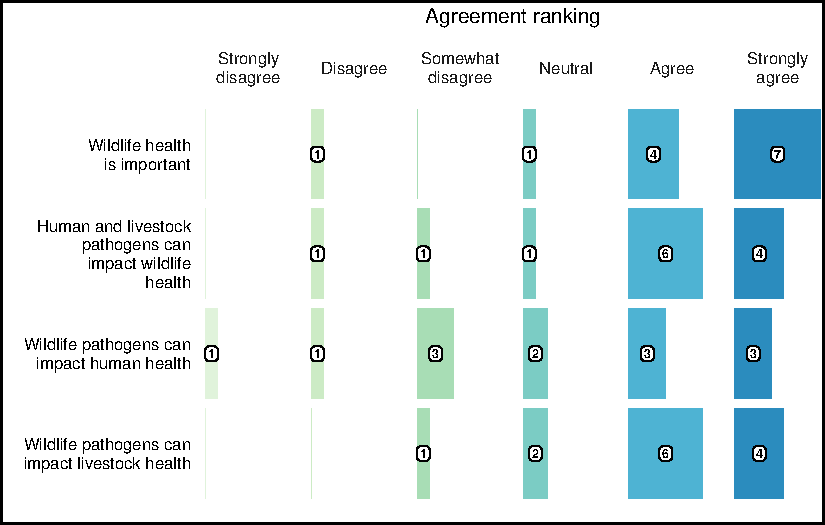
\includegraphics{Appendix_final_files/figure-pdf/section 1 plot-1.pdf}

}

\caption{Distribution of the level of agreement among protected area
data managers with statements `wildlife health is important to achieve
the conservation goals of protected area(s) where I work in' (row 1),
`human or livestock pathogens can affect wildlife populations inhabiting
the protected area(s) where I work in' (row 2), `pathogens carried by
wildlife inhabiting the protected area(s) where I work in can affect
human health' (row 3), and `pathogens carried by wildlife inhabiting the
protected area(s) where I work in can affect livestock health' (row 4).}

\end{figure}

\hypertarget{section-2-overall-frequency-of-encounters-with-dead-sick-or-injured-wildlife-in-protected-areas-and-their-documentation-when-found-during-patrols}{%
\subsubsection{Section 2: Overall frequency of encounters with dead,
sick, or injured wildlife in protected areas and their documentation
when found during
patrols}\label{section-2-overall-frequency-of-encounters-with-dead-sick-or-injured-wildlife-in-protected-areas-and-their-documentation-when-found-during-patrols}}

\begin{figure}[H]

{\centering 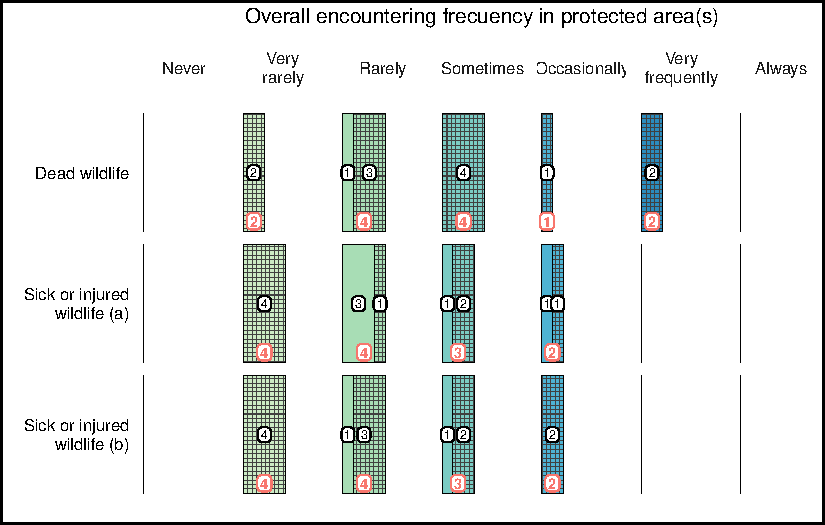
\includegraphics{Appendix_final_files/figure-pdf/section 2A plot-1.pdf}

}

\caption{Distribution of protected area data manager responses regarding
the encounter of dead and sick or injured wildlife in the protected
area(s) where they work. Red numbers indicate the total number of
responses per encountering frequency. The dashed area of the polygons
represent the responses indicating that dead, sick, and injured wildlife
found during ranger patrols are recorded (rows 1 -- 3, respectively).
Black numbers indicate the total number of responses reporting recording
and non-recording of dead, sick, and injured wildlife found during
patrols per encountering frequency.}

\end{figure}

\begin{figure}[H]

{\centering 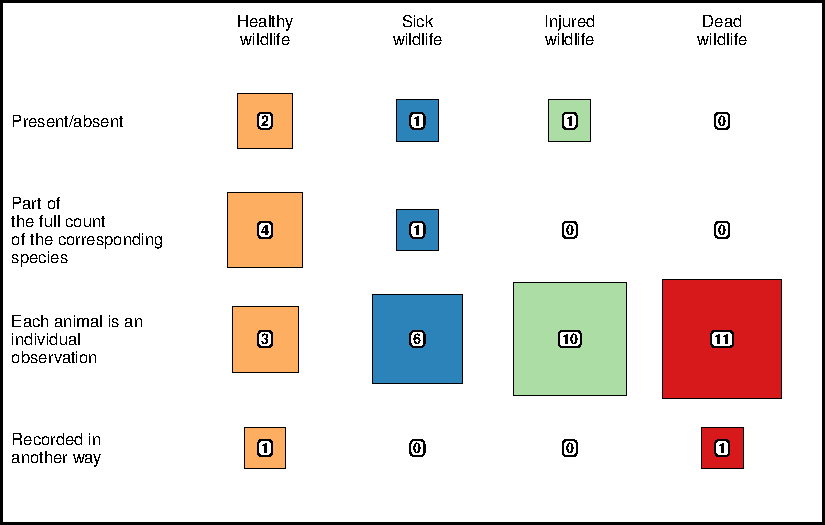
\includegraphics{Appendix_final_files/figure-pdf/section 2D plot-1.pdf}

}

\caption{Distribution of methods of documentation to register either
sick, injured, or dead wildlife found during ranger patrols reported by
protected area data managers.}

\end{figure}

\begin{figure}[H]

{\centering 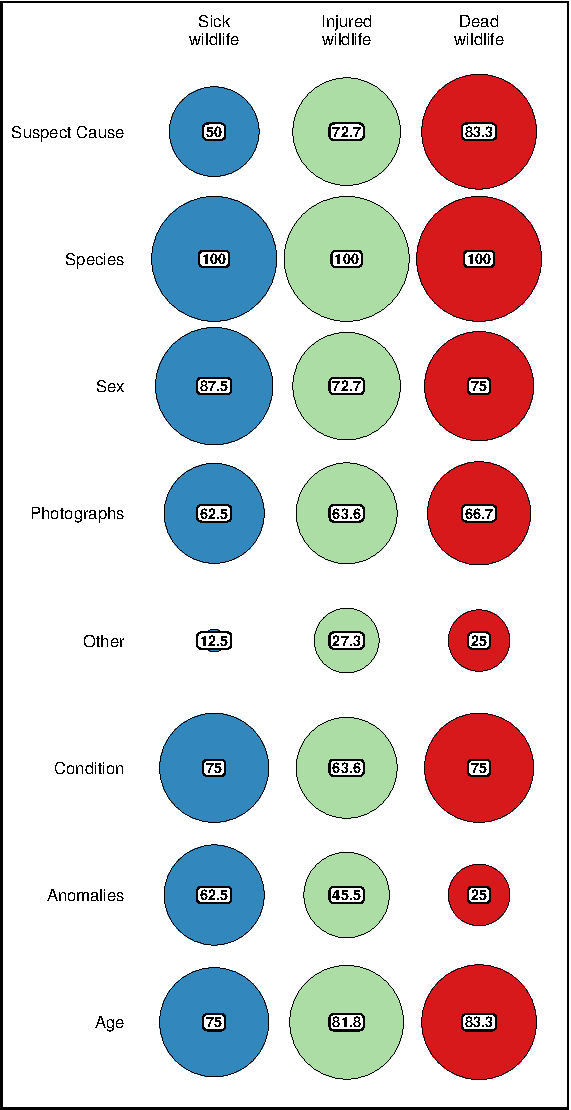
\includegraphics{Appendix_final_files/figure-pdf/data items collected-1.pdf}

}

\caption{The percentage of protected area data manager responses
indicating the documentation of sick, injured, and dead wildlife found
during patrols that record specific data items for each wildlife health
status. The size of the circles is proportional to the percentages
observed.}

\end{figure}

\hypertarget{section-3-presence-of-domestic-animals-in-protected-areas-the-documentation-of-their-health-status-and-the-perceived-threats-of-domestic-animals-to-conservation-goals}{%
\subsubsection{Section 3: Presence of domestic animals in protected
areas, the documentation of their health status, and the perceived
threats of domestic animals to conservation
goals}\label{section-3-presence-of-domestic-animals-in-protected-areas-the-documentation-of-their-health-status-and-the-perceived-threats-of-domestic-animals-to-conservation-goals}}

\begin{figure}[H]

{\centering 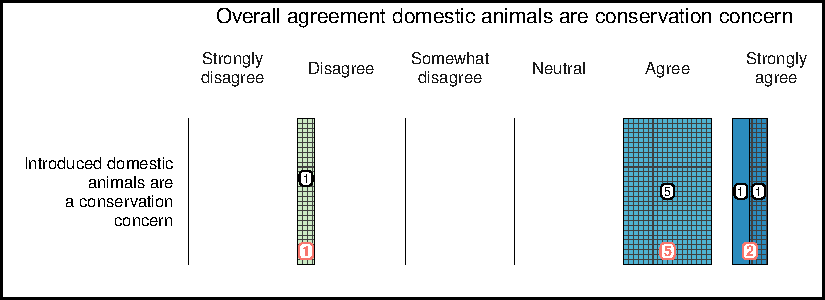
\includegraphics{Appendix_final_files/figure-pdf/plot appendix section 3-1.pdf}

}

\caption{Distribution of the level of agreement among protected area
data managers with the statement `introduced domestic animals (e.g.,
dogs, cats, cattle, pigs, cats) are a concern for the conservation goals
of the protected areas where I work'. Red numbers indicate the total
number of responses per agreement. The dashed area of the polygons
represent the responses indicating that domestic animals found during
ranger patrols are recorded. Black numbers indicate the total number of
responses reporting documentation and non-documentation of domestic
animals found during patrols.}

\end{figure}

\hypertarget{section-4-health-data-storage-practices-in-protected-areas}{%
\subsubsection{Section 4: Health data storage practices in protected
areas}\label{section-4-health-data-storage-practices-in-protected-areas}}

\begin{figure}[H]

{\centering 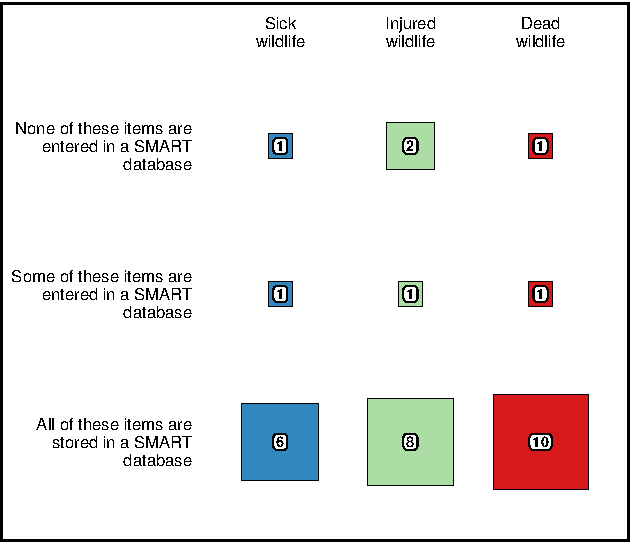
\includegraphics{Appendix_final_files/figure-pdf/plot health data storage practices-1.pdf}

}

\caption{Distribution of protected area data managers reporting the
documentation of either sick, injured, or dead wildlife found during
ranger patrols across data storage practices with respect to the use of
SMART.}

\end{figure}

\hypertarget{section-5-current-state-of-smart-deployment-in-protected-areas}{%
\subsubsection{Section 5: Current state of SMART deployment in protected
areas}\label{section-5-current-state-of-smart-deployment-in-protected-areas}}

Ten protected area data managers reported that SMART was fully
rolled-out, and 3 partially rolled-out. The most common SMART Desktop
version by the time of the survey was SMART 6, reported by 5 data
managers. SMART 7 was already available for 5 data managers by the time
of the survey. Older SMART versions were reported once. Finally, 9 data
managers reported SMART Connect availability and 1 mentioned plans to
set it up.

\newpage{}

\hypertarget{comparing-the-results-of-non-local-and-local-responses-from-the-same-country}{%
\subsection{Comparing the results of non-local and local responses from
the same
country}\label{comparing-the-results-of-non-local-and-local-responses-from-the-same-country}}

\hypertarget{section-1-perceptions-regarding-wildlife-health-importance-in-conservation-and-potential-consequences-of-pathogen-transmission-among-wildlife-domestic-animals-and-people-in-local-surveys-and-non-local-surveys-containing-protected-areas-in-local-responses}{%
\subsubsection{Section 1: Perceptions regarding wildlife health
importance in conservation and potential consequences of pathogen
transmission among wildlife, domestic animals, and people in local
surveys and non-local surveys containing protected areas in local
responses}\label{section-1-perceptions-regarding-wildlife-health-importance-in-conservation-and-potential-consequences-of-pathogen-transmission-among-wildlife-domestic-animals-and-people-in-local-surveys-and-non-local-surveys-containing-protected-areas-in-local-responses}}

\begin{table}[H]

\caption{Non-local and local responses for section 1 in country 1}
\centering
\begin{tabular}[t]{>{\raggedright\arraybackslash}p{2cm}|>{\raggedright\arraybackslash}p{3cm}|>{\raggedright\arraybackslash}p{3cm}|>{\raggedright\arraybackslash}p{3cm}|>{\raggedright\arraybackslash}p{3cm}}
\hline
Response
category & Wildlife health
is important & Human and livestock
pathogens can
impact wildlife
health & Wildlife pathogens can
impact human health & Wildlife pathogens can
impact livestock health\\
\hline
Global & Agree & Agree & Agree & Neutral\\
\hline
Local & Strongly agree & Agree & Agree & \vphantom{1} Agree\\
\hline
Local & Strongly agree & Strongly agree & Strongly agree & Strongly agree\\
\hline
Local & Strongly agree & Agree & Strongly agree & Agree\\
\hline
Local & Strongly agree & Agree & Agree & Agree\\
\hline
\end{tabular}
\end{table}

\begin{table}[H]

\caption{Non-local and local responses for section 1 in country 2}
\centering
\begin{tabular}[t]{>{\raggedright\arraybackslash}p{2cm}|>{\raggedright\arraybackslash}p{3cm}|>{\raggedright\arraybackslash}p{3cm}|>{\raggedright\arraybackslash}p{3cm}|>{\raggedright\arraybackslash}p{3cm}}
\hline
Response
category & Wildlife health
is important & Human and livestock
pathogens can
impact wildlife
health & Wildlife pathogens can
impact human health & Wildlife pathogens can
impact livestock health\\
\hline
Global & Neutral & Agree & Agree & Somewhat Disagree\\
\hline
Local & Strongly agree & Strongly agree & Strongly agree & Strongly agree\\
\hline
\end{tabular}
\end{table}

\begin{table}[H]

\caption{Non-local and local responses for section 1 in country 3}
\centering
\begin{tabular}[t]{>{\raggedright\arraybackslash}p{2cm}|>{\raggedright\arraybackslash}p{3cm}|>{\raggedright\arraybackslash}p{3cm}|>{\raggedright\arraybackslash}p{3cm}|>{\raggedright\arraybackslash}p{3cm}}
\hline
Response
category & Wildlife health
is important & Human and livestock
pathogens can
impact wildlife
health & Wildlife pathogens can
impact human health & Wildlife pathogens can
impact livestock health\\
\hline
Global & Strongly agree & Strongly agree & Strongly agree & Strongly agree\\
\hline
Global & Disagree & Strongly agree & Neutral & Strongly disagree\\
\hline
Local & Agree & Neutral & Neutral & Neutral\\
\hline
Local & Agree & Agree & Agree & \vphantom{1} Agree\\
\hline
Local & Agree & Agree & Somewhat Disagree & Somewhat Disagree\\
\hline
Local & Agree & Strongly agree & Neutral & Strongly \vphantom{1} agree\\
\hline
Local & Strongly agree & Strongly agree & Strongly agree & Strongly \vphantom{2} agree\\
\hline
Local & Strongly agree & Strongly agree & Agree & Agree\\
\hline
Local & Agree & Agree & Somewhat Disagree & Agree\\
\hline
Local & Strongly agree & Disagree & Strongly disagree & Strongly agree\\
\hline
Local & Strongly agree & Strongly agree & Disagree & Agree\\
\hline
Local & Agree & Strongly agree & Neutral & Agree\\
\hline
Local & Agree & Disagree & Neutral & Agree\\
\hline
Local & Agree & Strongly agree & Strongly disagree & Strongly disagree\\
\hline
Local & Strongly agree & Strongly agree & Disagree & Disagree\\
\hline
Local & Agree & Agree & Agree & Agree\\
\hline
Local & Agree & Strongly agree & Neutral & Strongly agree\\
\hline
Local & Strongly agree & Agree & Neutral & \vphantom{1} Neutral\\
\hline
Local & Strongly agree & Strongly agree & Strongly agree & Strongly \vphantom{1} agree\\
\hline
Local & Agree & Neutral & Neutral & Agree\\
\hline
Local & Strongly agree & Strongly agree & Strongly agree & Strongly agree\\
\hline
Local & Strongly agree & Agree & Agree & Strongly agree\\
\hline
Local & Agree & Agree & Strongly agree & Agree\\
\hline
Local & Strongly agree & Strongly agree & Strongly disagree & Strongly disagree\\
\hline
Local & Strongly agree & Agree & Neutral & Neutral\\
\hline
Local & Strongly agree & Neutral & Somewhat Disagree & Somewhat Disagree\\
\hline
\end{tabular}
\end{table}

\begin{table}[H]

\caption{Non-local and local responses for section 1 in country 4}
\centering
\begin{tabular}[t]{>{\raggedright\arraybackslash}p{2cm}|>{\raggedright\arraybackslash}p{3cm}|>{\raggedright\arraybackslash}p{3cm}|>{\raggedright\arraybackslash}p{3cm}|>{\raggedright\arraybackslash}p{3cm}}
\hline
Response
category & Wildlife health
is important & Human and livestock
pathogens can
impact wildlife
health & Wildlife pathogens can
impact human health & Wildlife pathogens can
impact livestock health\\
\hline
Global & Strongly agree & Strongly agree & Agree & Strongly agree\\
\hline
Local & Strongly agree & Strongly agree & Strongly agree & Strongly agree\\
\hline
Local & Strongly agree & Strongly agree & Neutral & Strongly agree\\
\hline
\end{tabular}
\end{table}

\hypertarget{section-2-overall-frequency-of-encounters-with-dead-sick-or-injured-wildlife-in-protected-areas-and-their-documentation-when-found-during-patrols-in-local-surveys-and-non-local-surveys-containing-protected-areas-in-local-responses}{%
\subsubsection{Section 2: Overall frequency of encounters with dead,
sick, or injured wildlife in protected areas and their documentation
when found during patrols in local surveys and non-local surveys
containing protected areas in local
responses}\label{section-2-overall-frequency-of-encounters-with-dead-sick-or-injured-wildlife-in-protected-areas-and-their-documentation-when-found-during-patrols-in-local-surveys-and-non-local-surveys-containing-protected-areas-in-local-responses}}

\begin{table}[H]

\caption{Non-local and local responses for section 2 in country 1}
\centering
\begin{tabular}[t]{>{\raggedright\arraybackslash}p{2cm}|>{\raggedright\arraybackslash}p{3cm}|>{\raggedright\arraybackslash}p{2cm}|>{\raggedright\arraybackslash}p{3cm}|>{\raggedright\arraybackslash}p{2cm}|>{\raggedright\arraybackslash}p{2cm}}
\hline
Response
category & Dead wildlife
encounter frequency & Dead wildlife
found in patrols
is recorded & Sick or injured wildlife
encounter frequency & Sick wildlife
found in patrols
is recorded & Injured wildlife
found in patrols
is recorded\\
\hline
Global & Sometimes & Yes & Sometimes & No & No\\
\hline
Local & Very frequently & Yes & Sometimes & Yes & Yes\\
\hline
Local & Very rarely & Yes & Very rarely & Yes & Yes\\
\hline
Local & Sometimes & Yes & Sometimes & Yes & \vphantom{1} Yes\\
\hline
Local & Sometimes & Yes & Sometimes & Yes & Yes\\
\hline
\end{tabular}
\end{table}

\begin{table}[H]

\caption{Non-local and local responses for section 2 in country 2}
\centering
\begin{tabular}[t]{>{\raggedright\arraybackslash}p{2cm}|>{\raggedright\arraybackslash}p{3cm}|>{\raggedright\arraybackslash}p{2cm}|>{\raggedright\arraybackslash}p{3cm}|>{\raggedright\arraybackslash}p{2cm}|>{\raggedright\arraybackslash}p{2cm}}
\hline
Response
category & Dead wildlife
encounter frequency & Dead wildlife
found in patrols
is recorded & Sick or injured wildlife
encounter frequency & Sick wildlife
found in patrols
is recorded & Injured wildlife
found in patrols
is recorded\\
\hline
Global & Rarely & No & Rarely & No & No\\
\hline
Local & Rarely & Yes & Occasionally & No & No\\
\hline
\end{tabular}
\end{table}

\begin{table}[H]

\caption{Non-local and local responses for section 2 in country 3}
\centering
\begin{tabular}[t]{>{\raggedright\arraybackslash}p{2cm}|>{\raggedright\arraybackslash}p{3cm}|>{\raggedright\arraybackslash}p{2cm}|>{\raggedright\arraybackslash}p{3cm}|>{\raggedright\arraybackslash}p{2cm}|>{\raggedright\arraybackslash}p{2cm}}
\hline
Response
category & Dead wildlife
encounter frequency & Dead wildlife
found in patrols
is recorded & Sick or injured wildlife
encounter frequency & Sick wildlife
found in patrols
is recorded & Injured wildlife
found in patrols
is recorded\\
\hline
Global & Occasionally & Yes & Very rarely & Yes & Yes\\
\hline
Global & Sometimes & Yes & Very rarely & Yes & Yes\\
\hline
Local & Very rarely & No & Very rarely & No & \vphantom{3} No\\
\hline
Local & Sometimes & Yes & Rarely & No & Yes\\
\hline
Local & Occasionally & Yes & Occasionally & Yes & No\\
\hline
Local & Very rarely & Yes & Very rarely & No & Yes\\
\hline
Local & Always & No & Never & No & No\\
\hline
Local & Sometimes & No & Rarely & No & No\\
\hline
Local & Sometimes & No & Occasionally & No & No\\
\hline
Local & Never & No & Never & No & No\\
\hline
Local & Very rarely & No & Very rarely & No & \vphantom{2} No\\
\hline
Local & Very rarely & Yes & Very rarely & Yes & Yes\\
\hline
Local & Very rarely & No & Sometimes & No & No\\
\hline
Local & Very rarely & Yes & Very rarely & No & \vphantom{1} No\\
\hline
Local & Occasionally & Yes & Very rarely & No & No\\
\hline
Local & Very rarely & No & Very rarely & Yes & No\\
\hline
Local & Very rarely & Yes & Very rarely & No & No\\
\hline
Local & Rarely & No & Rarely & Yes & Yes\\
\hline
Local & Very frequently & Yes & Very frequently & No & Yes\\
\hline
Local & Occasionally & Yes & Sometimes & Yes & Yes\\
\hline
Local & Very frequently & Yes & Very frequently & Yes & Yes\\
\hline
Local & Sometimes & Yes & Rarely & No & No\\
\hline
Local & Rarely & Yes & Never & No & No\\
\hline
Local & Occasionally & Yes & Very rarely & No & Yes\\
\hline
Local & Very rarely & No & Very rarely & No & \vphantom{1} No\\
\hline
Local & Very rarely & No & Very rarely & No & No\\
\hline
\end{tabular}
\end{table}

\begin{table}[H]

\caption{Non-local and local responses for section 2 in country 4}
\centering
\begin{tabular}[t]{>{\raggedright\arraybackslash}p{2cm}|>{\raggedright\arraybackslash}p{3cm}|>{\raggedright\arraybackslash}p{2cm}|>{\raggedright\arraybackslash}p{3cm}|>{\raggedright\arraybackslash}p{2cm}|>{\raggedright\arraybackslash}p{2cm}}
\hline
Response
category & Dead wildlife
encounter frequency & Dead wildlife
found in patrols
is recorded & Sick or injured wildlife
encounter frequency & Sick wildlife
found in patrols
is recorded & Injured wildlife
found in patrols
is recorded\\
\hline
Global & Very frequently & Yes & Sometimes & Yes & Yes\\
\hline
Local & Always & Yes & Occasionally & Yes & Yes\\
\hline
Local & Occasionally & Yes & Rarely & No & No\\
\hline
\end{tabular}
\end{table}

\hypertarget{section-3-presence-of-domestic-animals-in-protected-areas-the-documentation-of-their-health-status-and-the-perceived-threats-of-domestic-animals-to-conservation-goals-in-local-surveys-and-non-local-surveys-containing-protected-areas-in-local-responses}{%
\subsubsection{Section 3: Presence of domestic animals in protected
areas, the documentation of their health status, and the perceived
threats of domestic animals to conservation goals in local surveys and
non-local surveys containing protected areas in local
responses}\label{section-3-presence-of-domestic-animals-in-protected-areas-the-documentation-of-their-health-status-and-the-perceived-threats-of-domestic-animals-to-conservation-goals-in-local-surveys-and-non-local-surveys-containing-protected-areas-in-local-responses}}

\begin{table}[H]

\caption{Non-local and local responses for section 3 in country 1}
\centering
\begin{tabular}[t]{>{\raggedright\arraybackslash}p{2cm}|>{\raggedright\arraybackslash}p{3cm}|>{\raggedright\arraybackslash}p{2cm}|>{\raggedright\arraybackslash}p{2cm}|>{\raggedright\arraybackslash}p{2cm}}
\hline
Response
category & Introduced domestic
animals are
a conservation
concern & Domestic animals
found in the
protected area & Domestic animals
are recorded & Domestic animals
health status
is recorded\\
\hline
Global & Agree & Yes & Yes & No\\
\hline
Local & Strongly agree & Yes & No \vphantom{1} & \\
\hline
Local & Agree & Yes & Yes & No\\
\hline
Local & Agree & Yes & No & \\
\hline
Local & Strongly agree & Yes & No & \\
\hline
\end{tabular}
\end{table}

\begin{table}[H]

\caption{Non-local and local responses for section 3 in country 2}
\centering
\begin{tabular}[t]{>{\raggedright\arraybackslash}p{2cm}|>{\raggedright\arraybackslash}p{3cm}|>{\raggedright\arraybackslash}p{2cm}|>{\raggedright\arraybackslash}p{2cm}|>{\raggedright\arraybackslash}p{2cm}}
\hline
Response
category & Introduced domestic
animals are
a conservation
concern & Domestic animals
found in the
protected area & Domestic animals
are recorded & Domestic animals
health status
is recorded\\
\hline
Global & Agree & Yes & Yes & No\\
\hline
Local & Agree & Yes & Yes & No\\
\hline
\end{tabular}
\end{table}

\begin{table}[H]

\caption{Non-local and local responses for section 3 in country 3}
\centering
\begin{tabular}[t]{>{\raggedright\arraybackslash}p{2cm}|>{\raggedright\arraybackslash}p{3cm}|>{\raggedright\arraybackslash}p{2cm}|>{\raggedright\arraybackslash}p{2cm}|>{\raggedright\arraybackslash}p{2cm}}
\hline
Response
category & Introduced domestic
animals are
a conservation
concern & Domestic animals
found in the
protected area & Domestic animals
are recorded & Domestic animals
health status
is recorded\\
\hline
Global & Strongly agree & Yes & Yes & No\\
\hline
Global & Strongly agree & Yes & No & \\
\hline
Local & Neutral & Yes & Yes & Yes\\
\hline
Local & Strongly agree & No &  \vphantom{3} & \\
\hline
Local & Neutral & Yes & Yes & \vphantom{2} No\\
\hline
Local & Somewhat Disagree & No &  & \\
\hline
Local & Strongly agree & Yes & Yes & \vphantom{1} No\\
\hline
Local & Agree & No &  \vphantom{1} & \\
\hline
Local & Agree & Yes & Yes & \vphantom{1} No\\
\hline
Local & Strongly disagree & No &  & \\
\hline
Local & Strongly agree & Yes & Yes & No\\
\hline
Local & Strongly agree & Yes & Yes & Yes\\
\hline
Local & Disagree & Yes & No & \\
\hline
Local & Agree & Yes & No \vphantom{1} & \\
\hline
Local & Strongly agree & No &  \vphantom{2} & \\
\hline
Local & Strongly agree & No &  \vphantom{1} & \\
\hline
Local & Strongly agree & No &  & \\
\hline
Local & Agree & Yes & Yes & No\\
\hline
Local & Neutral & Yes & Yes & \vphantom{1} No\\
\hline
Local & Neutral & No &  & \\
\hline
Local & Strongly agree & Yes & No \vphantom{1} & \\
\hline
Local & Agree & Yes & Yes & Yes\\
\hline
Local & Neutral & Yes & Yes & No\\
\hline
Local & Strongly agree & Yes & No & \\
\hline
Local & Agree & Yes & No & \\
\hline
Local & Agree & No &  & \\
\hline
\end{tabular}
\end{table}

\begin{table}[H]

\caption{Non-local and local responses for section 3 in country 4}
\centering
\begin{tabular}[t]{>{\raggedright\arraybackslash}p{2cm}|>{\raggedright\arraybackslash}p{3cm}|>{\raggedright\arraybackslash}p{2cm}|>{\raggedright\arraybackslash}p{2cm}|>{\raggedright\arraybackslash}p{2cm}}
\hline
Response
category & Introduced domestic
animals are
a conservation
concern & Domestic animals
found in the
protected area & Domestic animals
are recorded & Domestic animals
health status
is recorded\\
\hline
Global & Neutral & No &  & \\
\hline
Local & Somewhat Disagree & No &  & \\
\hline
Local & Neutral & No &  & \\
\hline
\end{tabular}
\end{table}

\hypertarget{section-4-health-data-storage-practices-in-local-surveys-and-non-local-surveys-containing-protected-areas-in-local-responses}{%
\subsubsection{Section 4: Health data storage practices in local surveys
and non-local surveys containing protected areas in local
responses}\label{section-4-health-data-storage-practices-in-local-surveys-and-non-local-surveys-containing-protected-areas-in-local-responses}}

\begin{table}[H]

\caption{Non-local and local responses for section 4 in country 1}
\centering
\begin{tabular}[t]{>{\raggedright\arraybackslash}p{2cm}|>{\raggedright\arraybackslash}p{2cm}|>{\raggedright\arraybackslash}p{2cm}|>{\raggedright\arraybackslash}p{2cm}|>{\raggedright\arraybackslash}p{2cm}|>{\raggedright\arraybackslash}p{2cm}|>{\raggedright\arraybackslash}p{2cm}}
\hline
Response
category & Dead wildlife
found in patrols
are recorded & Dead willdife
data in SMART & Sick wildlife
found in patrols
are recorded & Sick willdife
data in SMART & Injured wildlife
found in patrols
is recorded & Injured willdife
data in SMART\\
\hline
Global & Yes & Some & No &  & No & \\
\hline
Local & Yes & Some & Yes & Some & Yes & \vphantom{3} Some\\
\hline
Local & Yes & Some & Yes & Some & Yes & \vphantom{2} Some\\
\hline
Local & Yes & Some & Yes & Some & Yes & \vphantom{1} Some\\
\hline
Local & Yes & Some & Yes & Some & Yes & Some\\
\hline
\end{tabular}
\end{table}

\begin{table}[H]

\caption{Non-local and local responses for section 4 in country 2}
\centering
\begin{tabular}[t]{>{\raggedright\arraybackslash}p{2cm}|>{\raggedright\arraybackslash}p{2cm}|>{\raggedright\arraybackslash}p{2cm}|>{\raggedright\arraybackslash}p{2cm}|>{\raggedright\arraybackslash}p{2cm}|>{\raggedright\arraybackslash}p{2cm}|>{\raggedright\arraybackslash}p{2cm}}
\hline
Response
category & Dead wildlife
found in patrols
are recorded & Dead willdife
data in SMART & Sick wildlife
found in patrols
are recorded & Sick willdife
data in SMART & Injured wildlife
found in patrols
is recorded & Injured willdife
data in SMART\\
\hline
Global & No &  & No &  & No & \\
\hline
Local & Yes & Some & No &  & No & \\
\hline
\end{tabular}
\end{table}

\begin{table}[H]

\caption{Non-local and local responses for section 4 in country 3}
\centering
\begin{tabular}[t]{>{\raggedright\arraybackslash}p{2cm}|>{\raggedright\arraybackslash}p{2cm}|>{\raggedright\arraybackslash}p{2cm}|>{\raggedright\arraybackslash}p{2cm}|>{\raggedright\arraybackslash}p{2cm}|>{\raggedright\arraybackslash}p{2cm}|>{\raggedright\arraybackslash}p{2cm}}
\hline
Response
category & Dead wildlife
found in patrols
are recorded & Dead willdife
data in SMART & Sick wildlife
found in patrols
are recorded & Sick willdife
data in SMART & Injured wildlife
found in patrols
is recorded & Injured willdife
data in SMART\\
\hline
Global & Yes & Some & Yes & Some & Yes & \vphantom{1} Some\\
\hline
Global & Yes & Some & Yes & Some & Yes & Some\\
\hline
Local & No &  & No &  & No \vphantom{8} & \\
\hline
Local & Yes & Some & No &  & Yes & \vphantom{2} Some\\
\hline
Local & Yes & Some & Yes & Some & No & \\
\hline
Local & Yes & Some & No &  & Yes & \vphantom{1} Some\\
\hline
Local & No &  & No &  & No \vphantom{7} & \\
\hline
Local & No &  & No &  & No \vphantom{6} & \\
\hline
Local & No &  & No &  & No \vphantom{5} & \\
\hline
Local & No &  & No &  & No \vphantom{4} & \\
\hline
Local & No &  & No &  & No \vphantom{3} & \\
\hline
Local & Yes & Some & Yes & Some & Yes & \vphantom{2} Some\\
\hline
Local & No &  & No &  & No \vphantom{2} & \\
\hline
Local & Yes & Some & No &  & No \vphantom{2} & \\
\hline
Local & Yes & Some & No &  & No \vphantom{1} & \\
\hline
Local & No &  & Yes & None & No & \\
\hline
Local & Yes & None & No &  & No \vphantom{1} & \\
\hline
Local & No &  & Yes & Some & Yes & Some\\
\hline
Local & Yes & None & No &  & Yes & None\\
\hline
Local & Yes & Some & Yes & Some & Yes & \vphantom{1} Some\\
\hline
Local & Yes & Some & Yes & Some & Yes & Some\\
\hline
Local & Yes & None & No &  & No & \\
\hline
Local & Yes & Some & No &  & No & \\
\hline
Local & Yes & Some & No &  & Yes & Some\\
\hline
Local & No &  & No &  & No \vphantom{1} & \\
\hline
Local & No &  & No &  & No & \\
\hline
\end{tabular}
\end{table}

\begin{table}[H]

\caption{Non-local and local responses for section 4 in country 4}
\centering
\begin{tabular}[t]{>{\raggedright\arraybackslash}p{2cm}|>{\raggedright\arraybackslash}p{2cm}|>{\raggedright\arraybackslash}p{2cm}|>{\raggedright\arraybackslash}p{2cm}|>{\raggedright\arraybackslash}p{2cm}|>{\raggedright\arraybackslash}p{2cm}|>{\raggedright\arraybackslash}p{2cm}}
\hline
Response
category & Dead wildlife
found in patrols
are recorded & Dead willdife
data in SMART & Sick wildlife
found in patrols
are recorded & Sick willdife
data in SMART & Injured wildlife
found in patrols
is recorded & Injured willdife
data in SMART\\
\hline
Global & Yes & Some & Yes & Some & Yes & Some\\
\hline
Local & Yes & Some & Yes & Some & Yes & Some\\
\hline
Local & Yes & Some & No &  & No & \\
\hline
\end{tabular}
\end{table}



\end{document}
